\subsection{Our Dynamic Frontier approach}
\label{sec:frontier}

The \textit{Naive-dynamic} approach processes all vertices in the graph until convergence. However, if a batch update $\Delta^{t-} \cup \Delta^{t+}$ is small compared to the total number of edges $|E|$, then it is expected that the ranks of only a few vertices change. Our proposed \textit{Dynamic Frontier} approach incorporates this aspect, and identifies affected vertices efficiently via an incremental process.

% Incremental Iteration Method for Fast PageRank Computation (2015): In this paper, Kim and Choi \cite{kim2015incremental} propose an asynchronous approach for computing PageRank combined with the standard approach for finding the affected set of vertices (like Desikan et al. \cite{rank-desikan05}).


\subsubsection{Explanation of the approach}
\label{sec:frontier-explanation}

Consider a batch update consisting of edge deletions $(u, v) \in \Delta^{t-}$ and insertions $(u, v) \in \Delta^{t+}$. We first initialize the rank of each vertex to that obtained in the previous snapshot of the graph.

\begin{figure*}[hbtp]
  \centering
  \subfigure[Initial graph]{
    \label{fig:about-df-01}
    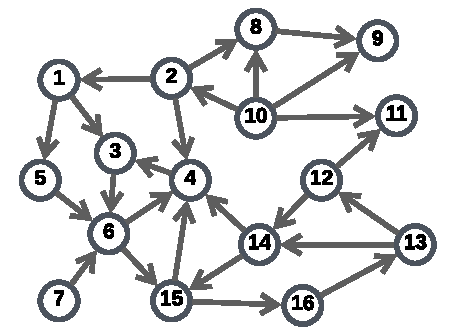
\includegraphics[width=0.23\linewidth]{out/about-df-01.pdf}
  }
  \subfigure[Marking affected (initial)]{
    \label{fig:about-df-02}
    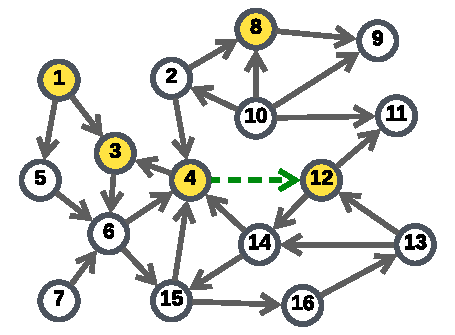
\includegraphics[width=0.23\linewidth]{out/about-df-02.pdf}
  }
  \subfigure[After first iteration]{
    \label{fig:about-df-03}
    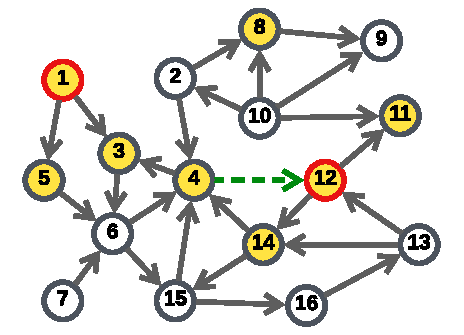
\includegraphics[width=0.23\linewidth]{out/about-df-03.pdf}
  }
  \subfigure[After second iteration]{
    \label{fig:about-df-04}
    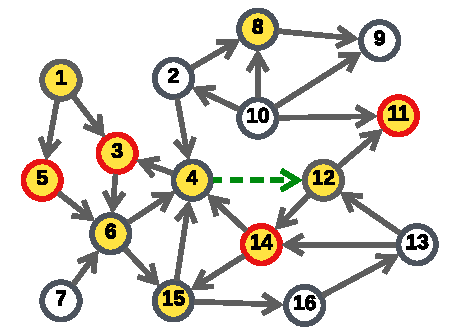
\includegraphics[width=0.23\linewidth]{out/about-df-04.pdf}
  } \\[-2ex]
  % \subfigure[]{
  %   \label{fig:about-df-05}
  %   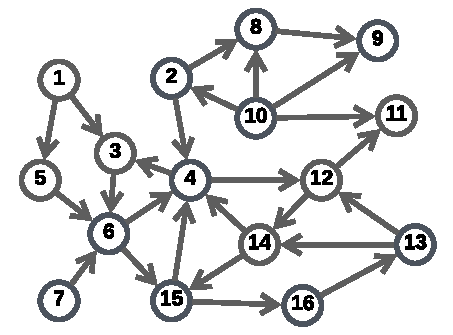
\includegraphics[width=0.18\linewidth]{out/about-df-05.pdf}
  % }
  \caption{Illustration of the \textit{Dynamic Frontier} approach through a specific example. The initial graph consists of $16$ vertices and $25$ edges. The graph is then updated with an edge insertion $(4, 12)$, and an edge deletion $(2, 1)$. Accordingly, the outgoing neighbors of vertices $4$ ($3$ and $12$) and $2$ ($1$, $4$, and $8$) are marked as affected (shown with yellow fill). When the ranks of these affected vertices are computed in the first iteration, it is found that change in rank of vertices $1$ and $12$ exceeds the frontier tolerance $\tau_f$ (shown with red border). Thus, outgoing neighbors of vertices $1$ ($3$ and $5$) and $12$ ($11$ and $14$) are also marked as affected. In the second iteration, the change in rank of vertices $3$, $5$, $11$, and $14$ is greater than $\tau_f$ --- thus their outgoing vertices are marked as affected. In the subsequent iteration, the ranks of affected vertices are again updated. If the change in rank of every vertex is within (iteration) tolerance $\tau$, the ranks of vertices have converged, and the algorithm terminates.}
  \label{fig:about-df}
\end{figure*}


\paragraph{Initial marking of affected vertex on edge deletion/insertion:}

For each edge deletion/insertion $(u, v)$, we initially mark the outgoing neighbors of the vertex $u$ in the previous $G^{t-1}$ and current graph snapshot $G^t$ as affected (lines \ref{alg:with-barrier--mark-begin}-\ref{alg:with-barrier--mark-end} in Algorithm \ref{alg:with-barrier}, and lines \ref{alg:barrier-free--mark-begin}-\ref{alg:barrier-free--mark-end} in Algorithm \ref{alg:barrier-free}).

\paragraph{Incremental marking of affected vertices upon change in rank of a given vertex:}

Next, while performing PageRank computation (lines \ref{alg:with-barrier--compute-begin}-\ref{alg:with-barrier--compute-end} in Algorithm \ref{alg:with-barrier}, and lines \ref{alg:barrier-free--compute-begin}-\ref{alg:barrier-free--compute-end} in Algorithm \ref{alg:barrier-free}), if the rank of any affected vertex $v$ changes in an iteration by an amount greater than the \textit{frontier tolerance} $\tau'$, we mark its outgoing neighbors as affected (lines \ref{alg:with-barrier--remark-begin}-\ref{alg:with-barrier--remark-end} in Algorithm \ref{alg:with-barrier}, and lines \ref{alg:barrier-free--remark-begin}-\ref{alg:barrier-free--remark-end} in Algorithm \ref{alg:barrier-free}). This process of marking vertices continues in every iteration.

\begin{algorithm}[!hbt]
\caption{Our parallel Dynamic Frontier PageRank.}
\label{alg:prdf}
\begin{algorithmic}[1]
\Require{$\Delta^{t-}, \Delta^{t+}$: Edge deletions and insertions (input)}
\Ensure{$R, R_{new}$: Previous, current rank vector}
\Ensure{$V_A[u]$: Is vertex $u$ affected due to current batch update?}

\Statex

\Function{dynamicFrontierPR}{$G^{t-1}, R^{t-1}, \Delta^{t-}, \Delta^{t+}$}
  \State $V_A \gets \{0\}$ \textbf{;} $R_{new} \gets R \gets R^{t-1}$
  \State $\rhd$ Mark initial affected
  \ForAll{$(u, v) \in \Delta^{t-} \cup \Delta^{t+} \textbf{in parallel}$} \label{alg:with-barrier--mark-begin}
    \ForAll{$v' \in (G^{t-1} \cup G^t).out(u)$}
    \State $V_A[v'] \gets 1$
    \EndFor
  \EndFor \label{alg:with-barrier--mark-end}
  % \State \textbf{wait for all threads} (implicit barrier)
  \ForAll{$i \in [0 .. MAX\_ITERATIONS)$} \label{alg:with-barrier--compute-begin}
    \ForAll{$v \in V^t$ \textbf{in parallel}}
      \State $\rhd$ Is vertex not affected?
      \If{$V_A[v] = 0$} \textbf{continue}
      \EndIf
      \State $r \gets (1 - \alpha)/|V^t|$
      \ForAll{$u \in G^t.in(v)$}
        \State $r \gets r + \alpha * R[u] / |G^t.out(u)|$
      \EndFor
      \State $\Delta r \gets |r - R[v]|$ \textbf{;} $R_{new}[v] \gets r$
      \State $\rhd$ Is rank change $>$ frontier tolerance?
      \If{$\Delta r > \tau'$} \label{alg:with-barrier--remark-begin}
        \ForAll{$v' \in G^t.out(v)$} $V_A[v'] \gets 1$
        \EndFor
      \EndIf \label{alg:with-barrier--remark-end}
    \EndFor
    % \State \textbf{wait for all threads} (implicit barrier)
    \State $\Delta R \gets l_\infty Norm(R, R_{new})$ \textbf{in parallel}
    \State $swap(R_{new}, R)$
    \State $\rhd$ Ranks converged?
    \If{$\Delta R \le \tau$} \textbf{break}
    \EndIf
  \EndFor \label{alg:with-barrier--compute-end}
  \State \ReturnInline{$R$}
\EndFunction
\end{algorithmic}
\end{algorithm}




%% Requires (parameters):
% G(V, E): a directed unweighted graph
% R: initial ranks (1/N for static)

%% Parameter values:
% MAX\_ITERATIONS = 500
% DAMPING\_FACTOR = 0.85
% TOLERANCE = 10^-10



\subsubsection{A simple example}

Figure \ref{fig:about-frontier} shows an example of the \textit{Dynamic Frontier} approach. The original graph, shown in Figure \ref{fig:about-frontier-01} consists of $16$ vertices. Subsequently, Figure \ref{fig:about-frontier-02} shows a batch update applied to the original graph involving the deletion of an edge from vertex $2$ to $1$ and the insertion of an edge from vertex $4$ to $12$. Following the batch update, we perform the initial step of the \textit{Dynamic Frontier} approach, marking outgoing neighbors of $2$ and $4$ as affected, i.e., $1$, $3$, $4$, $8$, and $12$ are marked as affected. Note that vertex $2$ is not affected as it is a source of the change while vertex $4$ being a neighbour of $2$ is also affected. Now, we are ready to execute the first iteration of PageRank algorithm.

During the first iteration (see Figure \ref{fig:about-frontier-03}), the ranks of affected vertices are updated. Consider that the change in rank of vertices $1$ and $12$ is observed to be greater than frontier tolerance $\tau'$, shown with red border in Figure \ref{fig:about-frontier-03}. In response to this, the \textit{Dynamic Frontier} approach incrementally marks the outgoing neighbors of $1$ and $12$ as affected, specifically vertices $5$, $11$, and $14$.

During the second iteration (see Figure \ref{fig:about-frontier-04}), the ranks of affected vertices are again updated. Further, consider that the change in rank of vertices $3$, $5$, $11$, and $14$ is observed to be greater than frontier tolerance $\tau'$, shown with red border in Figure \ref{fig:about-frontier-03}. As before, we mark the outgoing neighbors of $3$, $5$, $11$, and $14$ as affected, namely vertices $4$, $6$, and $15$.

In the subsequent iteration, the ranks of affected vertices are again updated. If the change in rank of every vertex is within (iteration) tolerance $\tau$, the ranks of vertices have converged, and the algorithm terminates.

% Illustration of the \textit{Dynamic Frontier} approach through a specific example. The initial graph consists of $16$ vertices and $25$ edges. The graph is then updated with an edge insertion $(4, 12)$, and an edge deletion $(2, 1)$. Accordingly, the outgoing neighbors of vertices $4$ ($3$ and $12$) and $2$ ($1$, $4$, and $8$) are marked as affected (shown with yellow fill). When the ranks of these affected vertices are computed in the first iteration, it is found that change in rank of vertices $1$ and $12$ exceeds the frontier tolerance $\tau_f$ (shown with red border). Thus, outgoing neighbors of vertices $1$ ($3$ and $5$) and $12$ ($11$ and $14$) are also marked as affected. In the second iteration, the change in rank of vertices $3$, $5$, $11$, and $14$ is greater than $\tau_f$ --- thus their outgoing vertices are marked as affected. In the subsequent iteration, the ranks of affected vertices are again updated. If the change in rank of every vertex is within (iteration) tolerance $\tau$, the ranks of vertices have converged, and the algorithm terminates.


\subsection{Dynamic Frontier With-barrier PageRank (\FroWbar{})}
\label{sec:frontier-withbarrier}

As mentioned in Section \ref{sec:withbarrier}, we perform a synchronous rank computation with \FroWbar{} using two rank vectors $R$, and $R_{new}$ (see Algorithm \ref{alg:with-barrier}).

\paragraph{Tracking affected vertices:}

To track vertices that are marked as affected due to the current batch update $\Delta^{t-} \cup \Delta^{t+}$, we use a flag vector $V_A$ (an 8-bit integer vector).

\paragraph{Detecting convergence:}

Note that $\Delta r$ represents the change in rank of single vertex, and $\Delta R$ represents the $L_\infty$-norm between the previous $R$ and the current rank vector $R_{new}$. When $\Delta R$ lies within (iteration) tolerance $\tau$, ranks are considered to have converged.



\subsection{Synchronous vs Asynchronous implementation}

We first want to check whether a synchronous, or an asynchronous implementation is suitable for \textit{Dynamic Frontier} PageRank. 
A synchronous implementation is one which uses two separate rank vectors, one as the input, and the other as the output --- at the end of each iteration, the vectors are swapped such that the output rank vector now becomes the input for the next iteration, and vice versa. This separation between the input and the output allows the results to be deterministic (for a parallel algorithm). On the other hand, an asynchronous implementation uses a single ranks vectors, and all updates are made in-place. This offers the possibility of faster convergence and absence of memory copies for unaffected/unprocessed vertices with dynamic approaches, but causes the results to be non-deterministic (for a parallel algorithm). To check whether a synchronous or an asynchronous implementation is suitable for \textit{Dynamic Frontier} PageRank, we attempt both the implementation for \textit{Static}, \textit{Naive-dynamic}, \textit{Dynamic Traversal}, and \textit{Dynamic Frontier} PageRank on batch updates (consisting purely of edge insertions; is this needed?) of size $10^{-7}|E|$ to $0.1|E|$. Figure \ref{fig:measure-affected} shows the average relative runtime with asynchronous implementations of \textit{Static}, \textit{Naive-dynamic}, \textit{Dynamic Traversal}, and \textit{Dynamic Frontier} PageRank compared to their respective synchronous implementations, on batch updates of size $10^{-7}|E|$ to $0.1|E|$ (right), and overall (left). The results indicate that asynchronous implementations are faster than synchronous ones, especially for smaller batch sizes. This is due to a somewhat faster convergence and the absence of copy overhead (for \textit{Dynamic Traversal} and \textit{Dynamic Frontier} approaches). Accordingly, we use the asynchronous implementations of \textit{Naive-dynamic}, \textit{Dynamic Traversal}, and \textit{Dynamic Frontier} PageRank.




\subsection{Determination of Frontier tolerance ($\tau_f$)}

We now wish to measure a suitable value for Frontier tolerance that allows us to minimize the number of vertices we process (after marking them as affected), while ensuring that we obtain ranks with the desired tolerance, i.e. we obtain ranks with no higher error than \textit{Static} PageRank for the same tolerance setting. For this, we adjust Frontier tolerance $\tau_f$ from $\tau$ to $\tau / 10^5$ and obtain ranks of vertices with the \textit{Dynamic Frontier} approach on batch updates (consisting purely of edge insertions) of size $10^{-7}|E|$ to $0.1|E|$. Figure \ref{fig:adjust-frontier} shows the average relative runtime and error in ranks obtained (with respect to ranks obtained with Reference Static PageRank) using \textit{Dynamic Frontier} approach. The figure indicates that increasing $\tau_f$ reduces runtime, but also increases the error. A Frontier tolerance $\tau_f$ of $\tau/10^4$ and $\tau/10^5$ obtain ranks with error lower than \textit{Static} PageRank, and are thus acceptable (we choose $\tau_f = \tau/10^5$ to be on the safe side).

\begin{figure*}[!hbt]
  \centering
  \subfigure{
    \label{fig:approach-async--mean}
    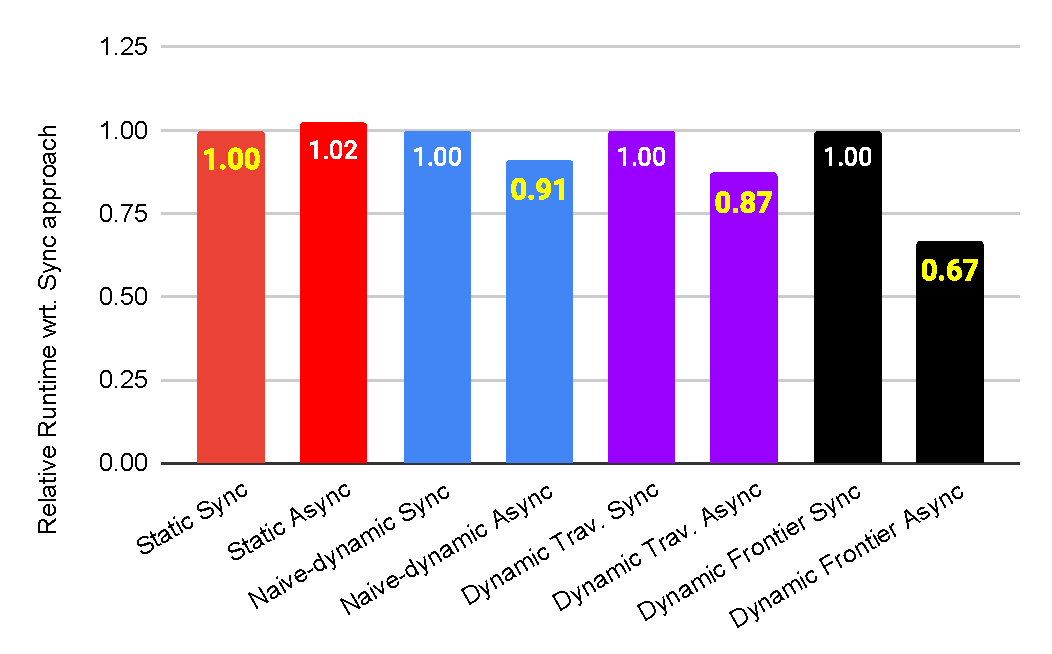
\includegraphics[width=0.48\linewidth]{out/approach-async-mean.pdf}
  }
  \subfigure{
    \label{fig:approach-async--batch}
    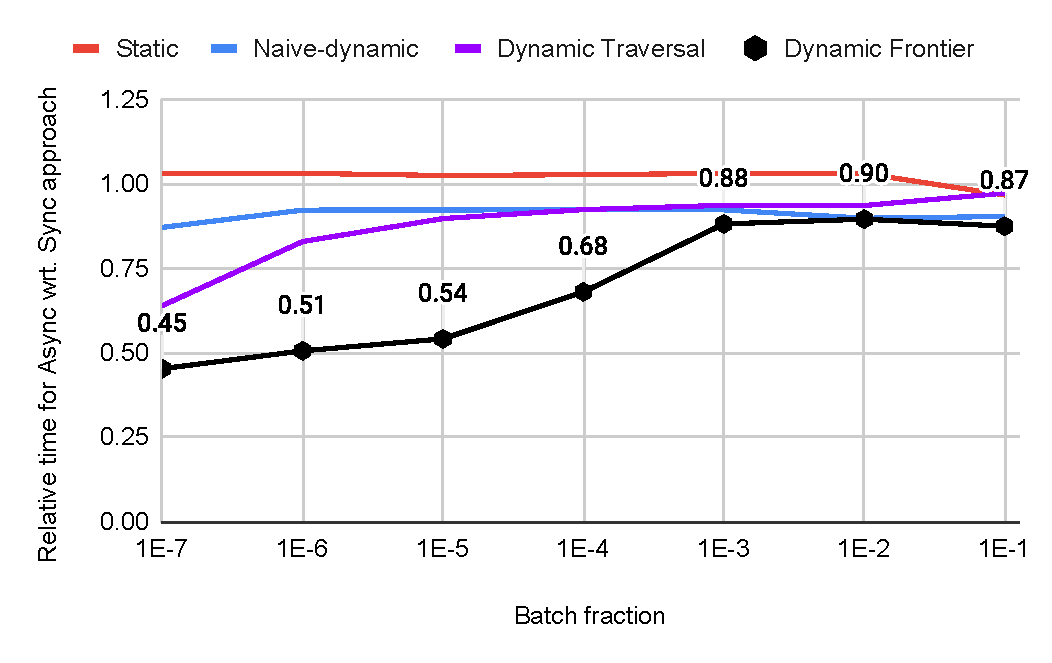
\includegraphics[width=0.48\linewidth]{out/approach-async-batch.pdf}
  } \\[-2ex]
  \caption{Average Relative runtime with asynchronous implementations of \textit{Static}, \textit{Naive-dynamic}, \textit{Dynamic Traversal}, and \textit{Dynamic Frontier} approach compared to their respective synchronous implementations, on batch updates of size $10^{-7}|E|$ to $0.1|E|$ (right), and overall (left). The results indicate that asynchronous implementations are faster than synchronous ones, especially for smaller batch sizes. This is due to a somewhat faster convergence and the absence of copy overhead (for \textit{Dynamic Traversal} and \textit{Dynamic Frontier} approaches).}
  \label{fig:approach-async}
\end{figure*}

\begin{figure}[!hbt]
  \centering
  \subfigure{
    \label{fig:adjust-frontier--runtime}
    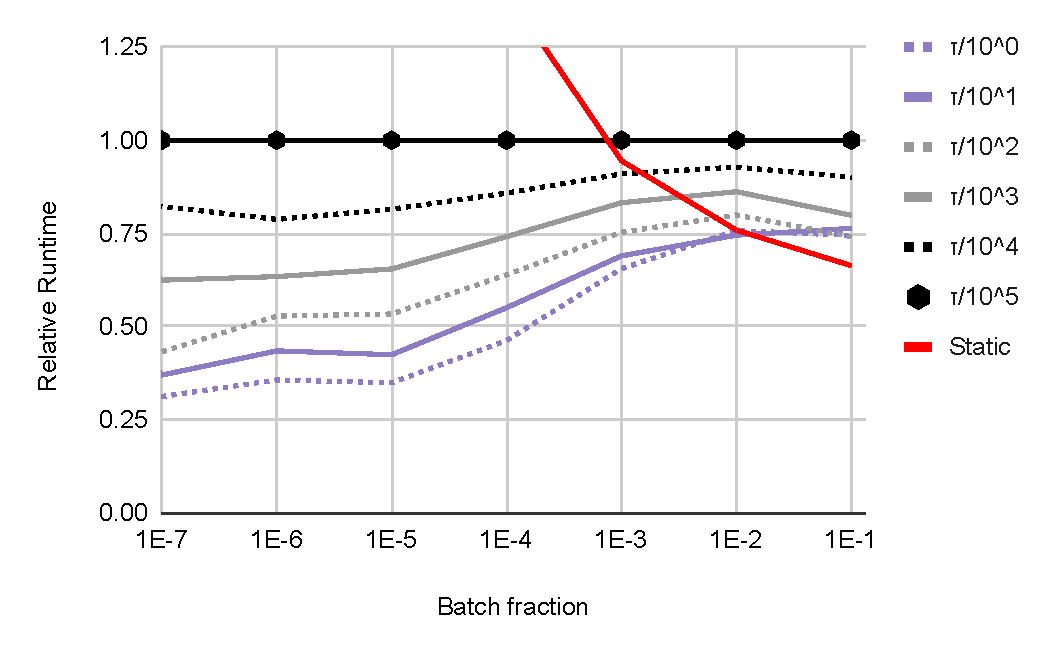
\includegraphics[width=0.98\linewidth]{out/adjust-frontier-runtime.pdf}
  } \\[-1ex]
  \subfigure{
    \label{fig:adjust-frontier--error}
    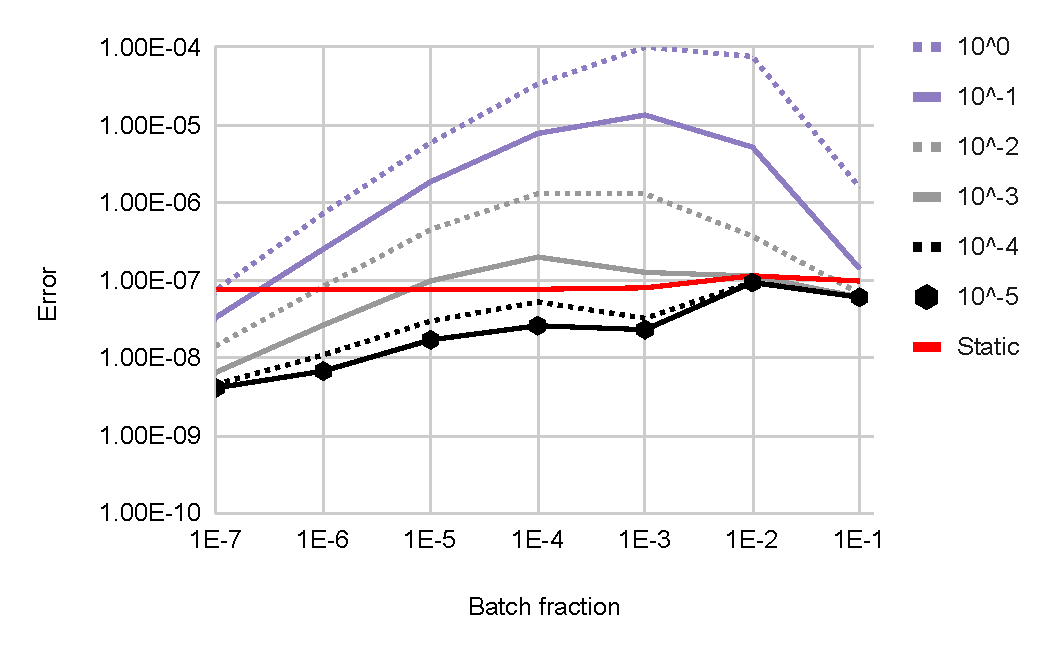
\includegraphics[width=0.98\linewidth]{out/adjust-frontier-error.pdf}
  } \\[-2ex]
\caption{Adjust Frontier. The error is averaged over the graphs in Table \ref{tab:dataset}.}
  \label{fig:adjust-frontier}
\end{figure}





% Dynamic Frontier (DF) approach
% Adjusting tolerance, Frontier tolerance, Mark DelRank / DelContrib
% Dynamic Frontier optimizations
% Edge-balanced approach (Chunk size)
